\section{Test}

Tale sezione ha lo scopo di spiegare il funzionamento, lo scopo e i risultati dei vari tipi di test proposti dal modello a V.

\subsection{Modello a V}
Il modello a V descrive in modo sintetico il ciclo di vita della realizzazione del software, partendo dalla sua progettazione fino alla sua consegna al cliente escludendo la fase di manutenzione.

Lo scopo del modello a V è quello di mostrare quali tipi di test accompagnano ogni fase del ciclo e di come anche questi siano propedeutici l'uno dall'altro.

\begin{figure}[H]
	\centering
	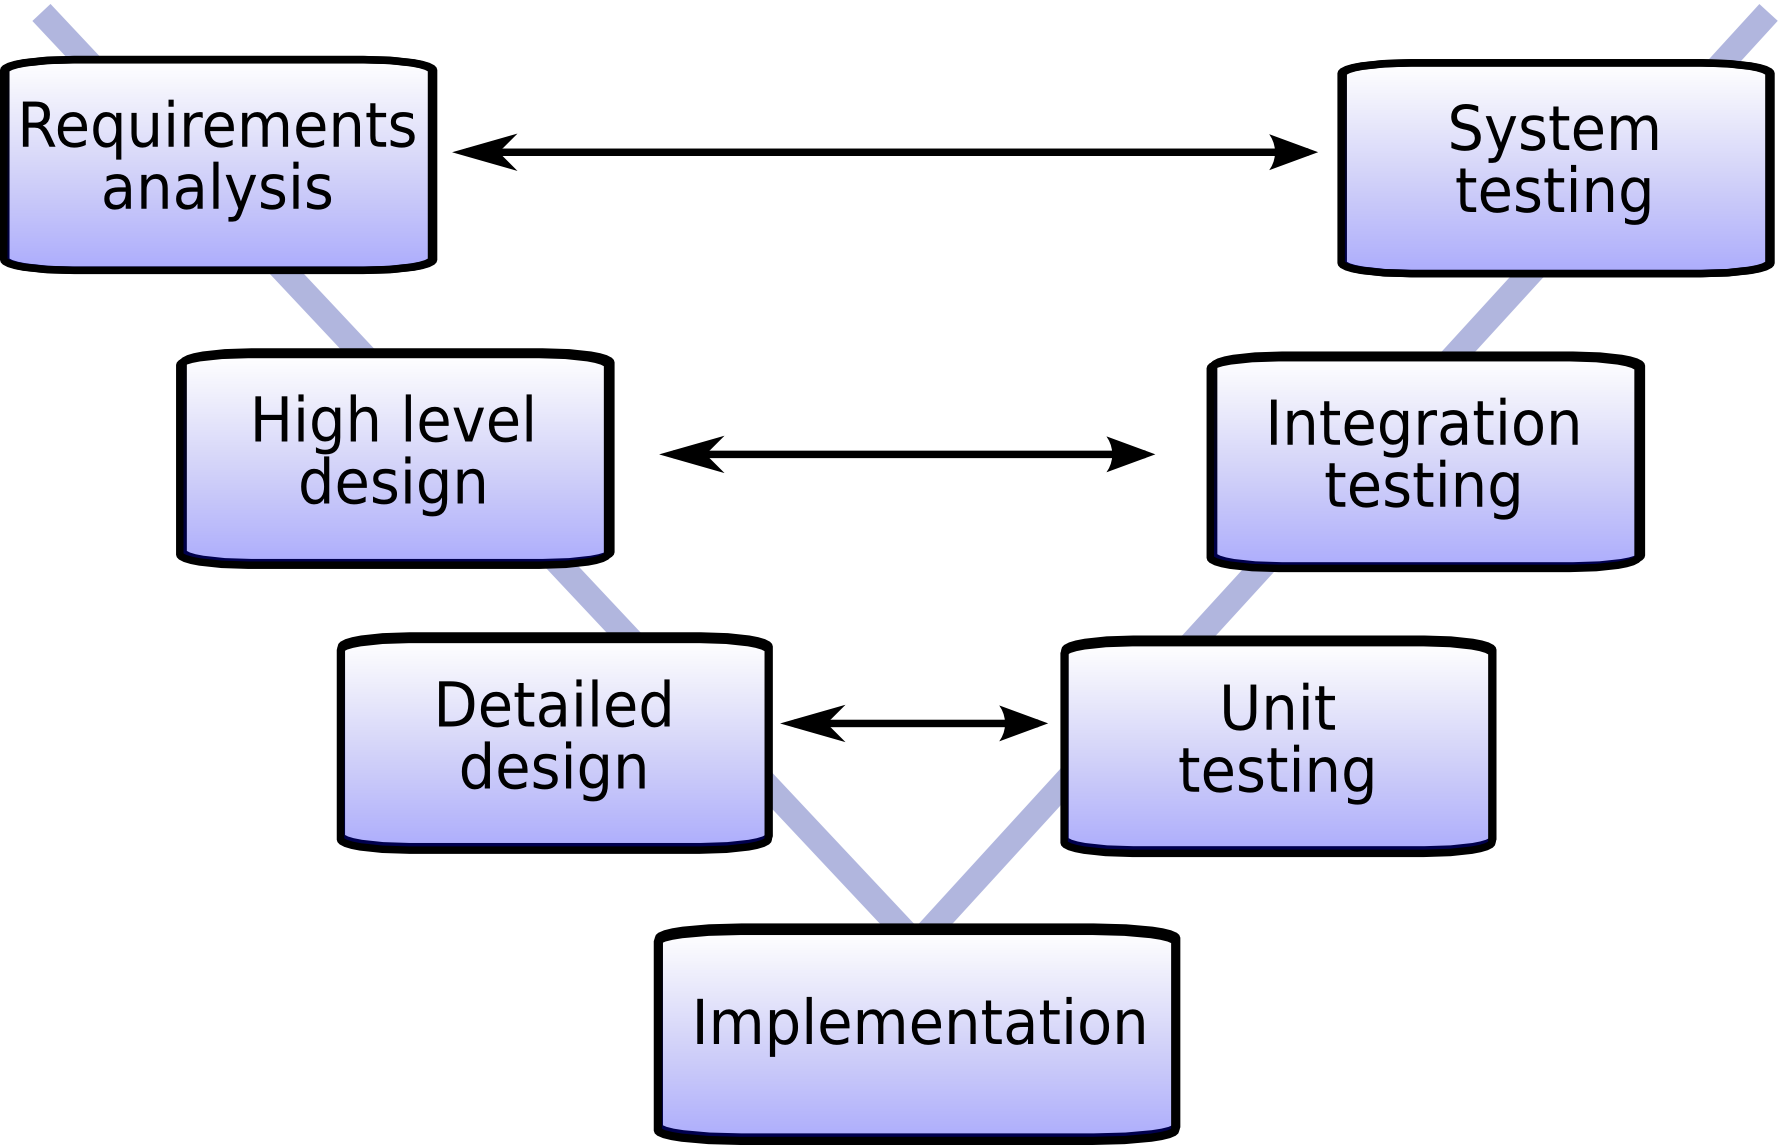
\includegraphics[width=0.5\textwidth]{img/V-model.png}
	\label{img:vmodel}
	\caption{Modello a V\protect\footnotemark}
\end{figure}

\footnotetext{Vedere Riferimenti Informativi in \S\ref{riferimenti informativi}}

\subsection{Classificazione e struttura dei test}
Le varie tipologie di test sono classificati nel seguente modo:

\begin{center}
	\texttt{T[Tipo][ID] [Nome]}
\end{center}

\begin{itemize}
	\item \textbf{Tipo}: la tipologia di test, seguendo il modello a V, sono:
	\begin{itemize}
		\item \textbf{S}: sistema
		\item \textbf{I}: integrazione.
		\item \textbf{U}: unità.
		\item \textbf{V}: validazione. %è la stessa cosa di collaudo e di accettazione??
	\end{itemize}
	\item \textbf{ID}: ogni tipologia di test prevede un numero incrementale di tre cifre che parte da uno.
	\item \textbf{Nome}: breve frase esplicativa che descrive lo scopo del test.
\end{itemize}

\subsection{Test di sistema}
Tipo di test da effettuare durante l'attività di analisi dei requisiti. Servono per svolgere la validazione del prodotto.

Come si può vedere dal modello a V, sono i primi tipi di test che vengono creati e saranno gli ultimi ad essere eseguiti prima della consegna del prodotto.

I test di sistema servono per testare l'intero prodotto, in particolare le sue specifiche tecniche e funzionali.
Per questo si creano dei test derivanti dai casi d'uso e dai requisiti funzionali presenti nell'\AdRd.

Per ogni test vengono affrontati i seguenti punti:

\begin{itemize}
	\item \textbf{Scopo}: lo scopo del test che; il titolo del punto non verrà inserito nei paragrafi dei test. %TODO: WHAT??
	\item \textbf{Procedura}: vengono descritti i passaggi da compiere per eseguire il test.
	\item \textbf{Approvazione}: vengono descritte le condizioni affinché il test sia considerato superato.
\end{itemize}

Alcuni termini ed espressioni assumono il seguente significato:

\begin{itemize}
	\item \textbf{Piattaforma di messaggistica}: s'intende sempre Telegram ed email.
	\item \textbf{Notifica}: s'intende una notifica in una delle piattaforme di messaggistica causata dall'applicazione.
	\item \textbf{Topic}: s'intende l'insieme delle etichette delle issue di GitLab e Redmine e delle keyword presenti nei messaggi di commit notificati dai push di GitLab.
	\item \textbf{Persona delegata}: s'intende l'utente a cui verranno inoltrate le notifiche nei giorni di indisponibilità dell'utente che sta usando l'applicazione. 
\end{itemize}

	\subsubsection{TS001 Inserimento utente}
		All'interno del gestore personale deve essere presente la possibilità di inserire e memorizzare la presenza di un nuovo utente che possa usare l'applicativo.
		
		\paragraph*{Procedura}
			\begin{enumerate}
				\item Inserire nel gestore personale le seguenti informazioni del nuovo utente:
				\begin{itemize}
					\item nome
					\item cognome
					\item contatto Telegram
					\item contatto email
				\end{itemize}
				
				\item Infine aggiungere l'utente.
			\end{enumerate}
	
		\paragraph*{Accettazione}
		Il nuovo utente deve comparire all'interno della lista degli utenti inseriti nell'applicazione.
	
	\subsubsection{TS002 Iscrizione ad una label, ad una piattaforma di messaggistica e apertura issue}
		Un utente quando s'iscrive ad una label, lo fa con l'intenzione di ricevere le notifiche inerenti solo a quella label provenienti da GitLab o Redmine e l'iscrizione alla piattaforma di messaggistica (Telegram o email) per scegliere dove ricevere tali notifiche.
		
		\paragraph*{Procedura}
			\begin{enumerate}
				\item Selezionare l'utente con cui si vuole usare l'applicativo.
				\item Selezionare la label da cui si vuole ricevere le notifiche. Dalle label è possibile capire quali notifiche derivano da Redmine e quali da GitLab.
				\item Selezionare Telegram o email per decidere in che piattaforma di messaggistica ricevere le notifiche della label.
				\item Aprire una issue da Gitlab se l'iscrizione è stata fatta da una label proveniente da GitLab, o aprire una issue da Redmine se l'iscrizione è stata fatta da una label proveniente da Redmine.
			\end{enumerate}
		
		\paragraph*{Accettazione}
		Alla piattaforma di messaggistica selezionata arriva una notifica dell'apertura della issue inerente al topic selezionato.
		
	\subsubsection{TS003 Iscrizione a una label, a una piattaforma di messaggistica e modifica issue}
		Come descritto nel test precedente, un utente può iscriversi a una label e a una piattaforma di messaggistica per ricevere una notifica.
		
		\paragraph*{Procedura}
			\begin{enumerate}
				\item Selezionare l'utente con cui si vuole usare l'applicativo.
				\item Selezionare la label da cui si vuole ricevere le notifiche. Dalla label è possibile capire quali derivano da Redmine e quali da GitLab.
				\item Selezionare Telegram o email per decidere in che piattaforma di messaggistica ricevere le notifiche delle label.
				\item Selezionare su Redmine, se ci si è iscritti ad una label di Redmine, o su GitLab, se ci si è inscritti ad una label su GitLab, una issue già aperta e modificarla in termini di label o titolo della issue.
				\item Se tra i campi modificati nella issue ci sono anche le label, iscriversi nel gestore personale alla label della issue modificata.
			\end{enumerate}
		
		\paragraph*{Accettazione}
		La modifica del titolo o delle label di una issue di Redmine o GitLab comporta l'invio della notifica a tutti gli iscritti alle nuove label, se queste sono cambiate, altrimenti agli iscritti delle solite label se è cambiato solo il titolo della issue. La modifica di qualsiasi altro campo non comporta l'invio di una notifica.
		
	\subsubsection{TS004 Disiscrizione da una label}
		La disiscrizione ad una label deve terminare la notifica delle segnalazioni legate a quella label.
		
		\paragraph*{Procedura}
			\begin{enumerate}
				\item Selezionare l'utente con cui si vuole usare l'applicativo.
				\item Disiscriversi da una label a cui precedentemente si era iscritti.
				\item Aprire o modificare una issue da Redmine o GitLab con la label da cui ci si è disiscritti precedentemente.
			\end{enumerate}
		
		\paragraph*{Accettazione}
		Una volta disiscritti ad una label non vengono più ricevute notifica riguardanti quella label.
		
	\subsubsection{TS005 Aggiunta di una keyword, iscrizione ad una piattaforma di messaggistica e push di Gitlab}
		Per ricevere le notifiche dei push di GitLab è possibile selezionare delle keyword che possono essere presenti nei messaggi di commit.
		
		\paragraph*{Procedura}
		\begin{itemize}
			\item Selezionare l'utente con cui si vuole usare l'applicativo.
			\item Aggiungere una keyword nel gestore personale.
			\item Effettuare un push su Gitlab dove il messaggio di commit contiene la keyword appena inserita.
		\end{itemize}
	
		\paragraph*{Accettazione}
		L'utente le notifiche dei push che nel loro messaggio di commit contengo la keyword aggiunta.
	
	\subsubsection{TS006 Rimozione di una keyword}
		La rimozione di una delle keyword aggiunta precedentemente evita di ricevere la notifica dei push di GitLab con il messaggio di commit con la keyword rimossa.
		
		\paragraph*{Procedura}
			\begin{enumerate}
				\item Selezionare l'utente con cui si vuole usare l'applicativo.
				\item Rimuovere una delle keyword selezionate in precedenza.
				\item Effettuare un push su GitLab dove il messaggio di commit contiene la keyword appena rimossa.
			\end{enumerate}
		
		\paragraph*{Accettazione}
		Non arrivano le notifiche dei push di Gitlab in cui nel messaggio di commit è presente la keyword appena rimossa.
		
	\subsubsection{TS007 Rimozione di una piattaforma di messaggistica}
		Come per il test precedente, anche rimuovendo una piattaforma di messaggistica (Telegram o email), le notifiche a quella piattaforma non dovrebbero più arrivare.
		
		\paragraph*{Procedura}
		\begin{enumerate}
			\item Selezionare l'utente con cui si vuole usare l'applicativo.
			\item Deselezionare una piattaforma di messaggistica precedentemente selezionata
			\item Creare o modificare una issue da Redmine o Gitlab, oppure effettuare un \gloss{push}. 
		\end{enumerate}
	
		\paragraph*{Accettazione}
		Dopo aver aperto una issue o effettuato un push da Gitlab o Redmine, non si ricevono più notifiche dalle piattaforme di messaggistica rimosse.
		
	\subsubsection{TS008 Aggiunta della persona delegata e dei giorni di indisponibilità}
		All'interno del gestore personale è possibile indicare i giorni di calendario in cui si è irreperibili ed è possibile selezionare una persona a cui inoltrare le notifiche che arrivano nei giorni selezionati.
		
		\paragraph*{Procedura}
			\begin{enumerate}
				\item Selezionare l'utente con cui si vuole usare l'applicativo.
				\item Aggiungere nel gestore personale il giorno di esecuzione del test come giorno di indisponibilità in cui non si vogliono ricevere notifiche dall'applicativo.
				\item Aggiungere, tra gli utenti inseriti nell'applicazione, l'utente a cui inoltrare le notifiche nei giorni di indisponibilità.
				\item Creare o modificare una issue da Redmine o Gitlab, oppure effettuare un \gloss{push}. 
			\end{enumerate}
		
		\paragraph*{Accettazione}
		La persona delegata riceve la notifica del messaggio che sarebbe dovuta arrivare all'utente che non è disponibile.
		
	\subsubsection{TS009 Rimozione giorni di indisponibilità}
		Nel momento in cui si rimuovono i giorni in cui ci si considera non reperibili, le notifiche dei topic a cui ci si è iscritti tornano ad essere inviate.
		
		\paragraph*{Procedura}
			\begin{enumerate}
				\item Selezionare l'utente con cui si vuole usare l'applicativo.
				\item Deselezionare tra i giorni di irreperibilità il giorno di esecuzione del test (se il giorno è già selezionato, selezionarlo e poi deselezionarlo).
				\item Effettuare un push da GitLab oppure aprire o modificare una issue su Redmine o GitLab.
			\end{enumerate}
		
		\paragraph*{Accettazione}
		L'utente selezionato ricomincia a ricevere notifiche.